%File: main.tex (AAAI-2026 anonymous submission)
\def\aaaianonymous{true}

\documentclass[letterpaper]{article} % DO NOT CHANGE THIS
\usepackage[submission]{aaai2026}  % DO NOT CHANGE THIS
\usepackage{times}  % DO NOT CHANGE THIS
\usepackage{helvet}  % DO NOT CHANGE THIS
\usepackage{courier}  % DO NOT CHANGE THIS
\usepackage[hyphens]{url}  % DO NOT CHANGE THIS
\usepackage{graphicx} % DO NOT CHANGE THIS
\urlstyle{rm} % DO NOT CHANGE THIS
\def\UrlFont{\rm}  % DO NOT CHANGE THIS
\usepackage{natbib}  % DO NOT CHANGE THIS
\usepackage{caption} % DO NOT CHANGE THIS
\frenchspacing  % DO NOT CHANGE THIS
\setlength{\pdfpagewidth}{8.5in} % DO NOT CHANGE THIS
\setlength{\pdfpageheight}{11in} % DO NOT CHANGE THIS

% Math / tables / theorems / figures
\usepackage{amsmath}
\usepackage{amssymb}
\usepackage{amsthm}
\usepackage{booktabs}
\usepackage{makecell}
\usepackage{pifont}
\usepackage{tikz}
\usetikzlibrary{arrows.meta,positioning,backgrounds,calc}
% Okabe-Ito colorblind-safe palette
\definecolor{oiVermillion}{HTML}{D55E00}
\definecolor{oiOrange}{HTML}{E69F00}
\definecolor{oiGreen}{HTML}{009E73}
\definecolor{oiBlue}{HTML}{0072B2}

\theoremstyle{plain}
\newtheorem{proposition}{Proposition}

\pdfinfo{
/TemplateVersion (2026.1)
}

\setcounter{secnumdepth}{0}

% Custom macros
\newcommand{\silr}{\textsc{SiLR}}
\newcommand{\psione}{\psi_1}
\newcommand{\psitwo}{\psi_2}
\newcommand{\psithree}{\psi_3}

\title{\silr{}: Structure-Preserving Admission and Process Reward for LLM Tool Agents}
\author{Anonymous Submission}
\affiliations{}

\begin{document}
\maketitle

\begin{abstract}
A runtime gate for an LLM tool-calling agent is usually cast as a filter, but in a ReAct loop a rejected proposal is followed by another at the same state, so the gate is in fact a \emph{search operator} over the agent's proposal stream---and the criterion it admits on shapes which trajectories are reachable. We study \emph{post-violation recovery admission}---admitting proposals that make progress toward recovery while the system is still in violation---and identify the \emph{scalar projection trap}: a gate that admits on an aggregate violation score collapses the multi-component violation geometry and commits the trajectory to a residual plateau, whereas a gate preserving a product order over the branch-level violation state (overloaded-branch support and per-branch severity) declines the geometry-poor step and keeps the search alive. We propose \silr{}, which shadow-executes each tool proposal and admits on this product order. On mined Gym-ANM scenarios, structured admission recovers $\mathbf{21/21}$ multi-action episodes where terminal admission deadlocks ($0/21$) and the best scalar slack reaches $9/21$, an advantage significant across the full $24$-scenario band; we prove the gap is a representational impossibility, and it holds across three model families and a second domain (CityLearn). Because the trust boundary is relocated from the LLM to the verifier, a magnitude-redistribution attack that defeats both scalar and support-only (Grid-Agent) baselines is contained only by the full per-branch predicate. The same geometry is structurally required at a \emph{second design point}: reused as a GRPO process reward it is a near-oracle, high-fidelity process signal---zero reward-level confusion versus $0.25$ for its count projection, dominating in all $24$ mined scenarios ($p{=}1.2{\times}10^{-7}$)---and the only reward under which the policy stays above the untrained base once the gate is removed ($0.844$ vs.\ $0.778$). Scalar projection loses the geometry at both design points; only the full product order is structurally sufficient.
\end{abstract}

\section{Introduction}
\label{sec:intro}

Critical infrastructures---power dispatch, datacenter scheduling, financial settlement---are increasingly automated by tool-using large language model (LLM) agents~\citep{gridagent2025}, and recent runtime-enforcement systems (SARC~\citep{sarc2026}, AgentSpec~\citep{agentspec2026}, GuardAgent~\citep{guardagent2025}, ShieldAgent~\citep{shieldagent2025}, VeriGuard~\citep{veriguard2025}) advance the runtime governance of these agents. These systems share an implicit premise: the system starts \emph{inside} the safe set and the gate's job is to keep it there. But infrastructure under autonomous control will sometimes start \emph{outside} it---already in violation, needing a multi-step sequence to recover---and there the enforcement question inverts: the gate must decide whether an action that still leaves the system unsafe nonetheless makes admissible progress toward recovery. This \emph{post-violation recovery admission} problem is structurally different from prevention and unaddressed by prior runtime governance for LLM tool agents; runtime mediation intercepts unsafe actions yet rarely converts blocked ones into safe completion~\citep{verifiertax2026}: enforcement is not recovery.

We frame the problem around \emph{admission semantics}: the formal criterion by which a runtime gate decides to apply or reject an LLM-proposed action. Our thesis is that this choice---not the gate's strictness---has first-order effects on whether multi-step recovery is possible. A terminal gate (admit only fully-recovered post-states) is safe but admits no intermediate step, deadlocking every multi-action episode on our mined Gym-ANM~\citep{henry2021gymanm} benchmark. The natural relaxation---a \emph{scalar admission gate} admitting any proposal whose aggregate violation penalty is non-increasing within a small slack---is structurally insufficient: relaxing its slack does not close the gap.

The reason is the \textbf{scalar projection trap}. In a ReAct loop a rejected proposal is followed by another at the same state, so \emph{the gate is not a filter but a search operator over the agent's proposal stream}; admitting on an aggregate score collapses the multi-component violation geometry and can commit the trajectory to a residual plateau from which recovery is unreachable under that gate, whereas a gate that preserves the per-branch geometry declines the geometry-poor step and keeps the search alive. The gap is representational, which we make precise as an impossibility result: structured admission recovers $\mathbf{21/21}$ multi-action episodes where terminal stalls at $0/21$ and the best scalar slack reaches $9/21$, an advantage significant across the full $24$-scenario band.

\paragraph{Contributions.} Our unifying claim is that one object---a product order over the branch-level violation state---is the right structure at \emph{two} design points of an LLM tool agent, and that projecting it to a scalar fails at both for the same representational reason.
\begin{itemize}\setlength{\itemsep}{1pt}
\item \textbf{The gate as a search operator, and the scalar projection trap.} We reframe a runtime admission gate from a filter into a search operator over the ReAct proposal stream, and characterize a failure mode of natural scalar recovery gates: admitting on an aggregate score collapses the multi-component violation geometry and can commit the trajectory to a residual plateau.
\item \textbf{Structured recovery admission (design point~1).} We propose \silr{}, a simulator-backed admission layer that shadow-executes each LLM tool proposal and admits it only when the product order is preserved, emitting graded \texttt{PASS}/\texttt{SAFE\_PROGRESS}/\texttt{FAIL} verdicts; we prove no scalar surrogate is sound with respect to this order.
\item \textbf{Empirical falsification across families and a second domain.} Terminal admission deadlocks and a scalar threshold sweep cannot close the gap; per-scenario plateau signatures and an MPC feasibility check confirm the mechanism is gate-induced. The dichotomy holds across three model families and reproduces in a second domain (CityLearn).
\item \textbf{Trust-boundary containment under LLM compromise.} Because admission is grounded in deterministic simulation, the trust boundary shifts to the verifier; a magnitude-redistribution attack that defeats both scalar admission and the Grid-Agent (support-only) baseline is contained only by the full per-branch predicate.
\item \textbf{The same geometry as a process reward (design point~2).} Reused as a GRPO signal the product order is a near-oracle, high-fidelity process reward---zero reward-level confusion against $0.25$ for its count projection---and the only reward under which the policy stays above the untrained baseline once the gate is removed; every tested scalar projection fails in at least one multi-family stress regime. This is the training-side counterpart of the admission-side impossibility.
\end{itemize}

\section{Related Work}
\label{sec:related}

\paragraph{Shielding and runtime guards.}
Shielding~\citep{alshiekh2018safe} synthesizes a finite-state shield from a temporal-logic specification that intercepts policy outputs at runtime; Model-Predictive Shielding~\citep{bastani2019mps}, Recovery RL~\citep{thananjeyan2021recovery}, and RL power-grid shielding~\citep{hrlshield2026} relax binary terminal gates by admitting recoverability-set states or screening actions with forward simulation, but all assume a fixed action space and require a backup/recovery policy or a dynamics-model lookahead. A parallel line adds runtime enforcement to tool-using LLM agents through architectural gates, guard agents, or rule languages---SARC's Pre-Action Gate~\citep{sarc2026} (the closest binary baseline, admitting a tool call only when a hand-written predicate holds), AgentSpec~\citep{agentspec2026}, GuardAgent~\citep{guardagent2025}, ShieldAgent~\citep{shieldagent2025}, and VeriGuard~\citep{veriguard2025}---yet none target post-violation recovery admission: a terminal predicate preserves safety but deadlocks multi-step recovery. \silr{} instead shields black-box LLM tool-call dispatch by single-step shadow simulation under a product order on the branch-level violation state, at constant per-step cost, making admission itself the design variable.

\paragraph{Grid-Agent and scalarization.}
Grid-Agent~\citep{gridagent2025} is the closest same-domain work: it couples LLM agents with sandboxed power-flow validation, rollback of negative actions, and monotonic-progress behavior for power-grid control. The mechanisms differ in kind: Grid-Agent's check is a \emph{post-hoc} rollback that reverts an action unless the violation set is resolved without introducing new violations---a support-level criterion with no per-branch severity guard---whereas \silr{}'s product order is a \emph{pre-action} admission predicate that never applies a geometry-poor step and emits graded verdicts reusable as a training signal. Scalarization trade-offs are classically a \emph{static} representational question~\citep{miettinen1999nonlinear}; our scalar projection trap is instead a \emph{behavioral} phenomenon of the runtime gate, which acts as a commitment operator over the ReAct proposal stream. Finally, where prompt-injection defenses~\citep{greshake2023injection} sanitize inputs or outputs, \silr{} assumes the LLM \emph{may} be compromised and enforces safety after the proposal by shadow execution, shifting the trust boundary from the LLM to the verifier. Table~\ref{tab:related} positions \silr{} against the closest systems along four axes---\emph{graded} admission, \emph{retained} multi-component violation geometry, \emph{black-box} LLM tool proposals, and the absence of any backup policy or dynamics lookahead---and it is the only point meeting all four.

\begin{table}[t]
\centering
\caption{Positioning of \silr{} against the closest runtime-safety systems. ``Geom.'': retains the (support, severity) violation state vs.\ a scalar aggregate; ``No look.'': single-step shadow only, no recovery policy or dynamics rollout.}
\label{tab:related}
\footnotesize
\setlength{\tabcolsep}{2pt}
\begin{tabular*}{\columnwidth}{@{\extracolsep{\fill}}lcccc@{}}
\toprule
System & Graded & Geom. & \makecell{Black-\\box LLM} & \makecell{No look-\\ahead} \\
\midrule
SARC Pre-Action Gate        & \ding{55} & \ding{55} & \ding{51} & \ding{51} \\
AgentSpec          & \ding{55} & \ding{55} & \ding{51} & \ding{51} \\
GuardAgent / ShieldAgent & \ding{55} & \ding{55} & \ding{51} & \ding{51} \\
Grid-Agent             & \ding{55} & \ding{55}$^\dagger$ & \ding{51} & \ding{55}$^\ddagger$ \\
MPS / Recovery RL & \ding{55} & \ding{55} & \ding{55} & \ding{55} \\
\silr{} (ours)                              & \ding{51} & \ding{51} & \ding{51} & \ding{51} \\
\bottomrule
\end{tabular*}\\[2pt]
{\footnotesize $^\dagger$support-level validation, no per-branch severity guard; $^\ddagger$applies then reverts (post-hoc rollback).}
\end{table}

\section{Threat Model and Method}
\label{sec:method}

\begin{figure*}[t]
\centering
\resizebox{0.72\textwidth}{!}{%
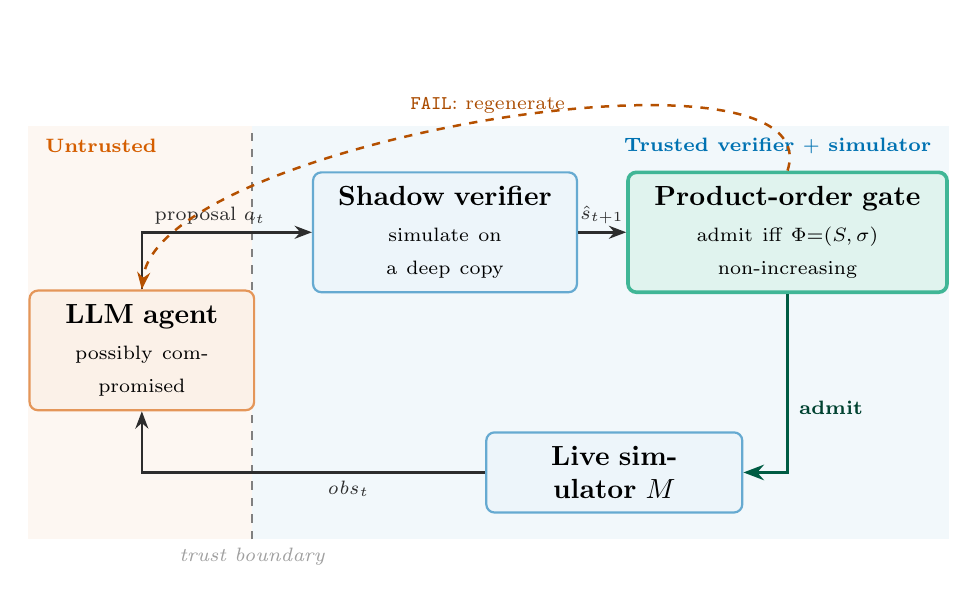
\begin{tikzpicture}[
  box/.style={rounded corners=3pt, draw, align=center, inner sep=5pt, line width=0.8pt},
  trusted/.style={fill=oiBlue!7, draw=oiBlue!60},
  untrusted/.style={fill=oiVermillion!9, draw=oiVermillion!65},
  hero/.style={fill=oiGreen!12, draw=oiGreen!75, line width=1.3pt},
  arr/.style={-{Stealth[length=2.2mm]}, line width=0.9pt, gray!35!black},
  admit/.style={-{Stealth[length=2.6mm]}, line width=1.4pt, oiGreen!58!black},
  fail/.style={-{Stealth[length=2.2mm]}, line width=0.9pt, oiVermillion!85!black, dashed},
  lbl/.style={font=\scriptsize, inner sep=1.5pt},
  lblg/.style={font=\scriptsize\bfseries, text=oiGreen!42!black, inner sep=1.5pt},
  lblr/.style={font=\scriptsize, text=oiVermillion!80!black, inner sep=1.5pt}
]
\node[box,untrusted,text width=2.5cm] (llm) at (0,0)
  {\textbf{LLM agent}\\[1pt]\scriptsize possibly compromised};
\node[box,trusted,text width=3.0cm] (shadow) at (3.85,1.5)
  {\textbf{Shadow verifier}\\[1pt]\scriptsize simulate on a deep copy};
\node[box,hero,text width=3.7cm] (gate) at (8.2,1.5)
  {\textbf{Product-order gate}\\[1pt]\scriptsize admit iff $\Phi{=}(S,\sigma)$ non-increasing};
\node[box,trusted,text width=2.9cm] (live) at (6.0,-1.55)
  {\textbf{Live simulator $M$}};
\begin{scope}[on background layer]
  \fill[oiVermillion!5] (-1.45,-2.4) rectangle (1.4,2.85);
  \fill[oiBlue!5] (1.4,-2.4) rectangle (10.25,2.85);
  \draw[dashed,gray,line width=0.8pt] (1.4,-2.4) -- (1.4,2.85);
\end{scope}
\node[gray!75,font=\scriptsize\itshape] at (1.4,-2.62) {trust boundary};
\node[oiVermillion,font=\scriptsize\bfseries,anchor=west] at (-1.35,2.6) {Untrusted};
\node[oiBlue,font=\scriptsize\bfseries,anchor=east] at (10.15,2.6) {Trusted verifier $+$ simulator};
\draw[arr] (llm.north) |- node[lbl,pos=0.7,above=1pt]{proposal $a_t$} (shadow.west);
\draw[arr] (shadow.east) -- node[lbl,above=1pt]{$\hat{s}_{t+1}$} (gate.west);
\draw[admit] (gate.south) |- node[lblg,pos=0.32,right=2pt]{admit} (live.east);
\draw[arr] (live.west) -| node[lbl,pos=0.2,below=1pt]{$\mathit{obs}_t$} (llm.south);
\draw[fail] (gate.north) to[out=72,in=84,looseness=0.58]
   node[lblr,pos=0.5,above=1pt]{\texttt{FAIL}: regenerate} (llm.north);
\end{tikzpicture}}
\caption{\silr{} admission architecture and trust boundary. A possibly-compromised LLM (untrusted) emits a tool proposal $a_t$; the verifier shadow-executes it on a deep copy of the trusted simulator, applies the product-order gate $\psi_1\wedge\psi_2\wedge\psi_3$, and either applies the admitted action ($\texttt{PASS}$/$\texttt{SAFE\_PROGRESS}$) or rejects it ($\texttt{FAIL}$, regenerating within the step).}
\label{fig:arch}
\end{figure*}

\paragraph{Trust boundary and adversary.}
\silr{} relocates the trust boundary from the LLM to the shadow simulator: no admission verdict depends on the LLM's reasoning, only on the simulator's deterministic response. The LLM is untrusted; the simulator, verifier, checkers, and tool layer are trusted. We adopt the compromised-prompt and compromised-observation capability class (the union of the SARC~\citep{sarc2026} and VeriGuard~\citep{veriguard2025} threat models): an attacker may (C1)~rewrite the system prompt, including operator-directive impersonation; (C2)~splice attacker-controlled text into every observation; and (C3)~persist both rewrites for the whole episode (worst case for the defender). The attacker may not modify the verifier, simulator, or tool-layer validators, bypass the tool-application interface, or read the verifier's shadow state. We score two safety failures---\emph{material worsening} (final penalty strictly above the no-intervention default) and \emph{false recovery} (terminal recovery reported while the live state still holds violations)---and their union, \emph{attack success}; recovery rate is reported separately as a liveness measure. Detailed attack constructions are deferred to the supplementary material.

\paragraph{Setting.}
An LLM tool-calling agent controls a critical-infrastructure simulator $M$ through a ReAct loop (Fig.~\ref{fig:arch}). At each control step $t=1,\ldots,C_{\text{step}}$ the agent observes $\mathit{obs}_t$, proposes a tool call $a_t$, and a runtime verifier mediates the proposal before it is applied; on rejection the agent regenerates within the same step, up to a per-step budget $C_{\text{prop}}$. \emph{Post-violation} initial conditions mean $M$ starts in $s_0$ with active constraint violations, and the goal is to drive $M$ violation-free. Two features make admission semantics central: a terminal gate stalls multi-action recovery, and---since a rejected proposal triggers another---the admitted nonterminal states shape which trajectories the agent explores.

\paragraph{Shadow-execution verifier.}
For each candidate $a_t$, the verifier evaluates a deterministic shadow state $\hat{s}_{t+1}=\mathrm{shadow}(s_t,a_t)=\mathrm{solve}(\mathrm{apply}(\mathrm{copy}(s_t),a_t))$, where $\mathrm{solve}(\cdot)$ is the domain's steady-state solver (Newton--Raphson power flow for Gym-ANM~\citep{henry2021gymanm}), run on a state-cloned copy of $M$ so rejected proposals leave the live system untouched.

\paragraph{Branch-level violation state and verdict ladder.}
We instantiate $\Phi$ on a vector-valued violation state; in our power-grid testbed the active family is branch loading, indexed by overloaded branch, and CityLearn instantiates the same construction on energy/comfort violations. Define the branch-level violation state
\begin{equation}
\Phi(s) = \bigl(S(s),\,\sigma(s)\bigr),
\quad S(s)\subseteq\mathcal{B},
\quad \sigma(s)\in\mathbb{R}_{\ge 0}^{|\mathcal{B}|},
\label{eq:phi}
\end{equation}
where $\mathcal{B}$ is the set of branches, $S(s)$ the support set of overloaded branches, and $\sigma(s)$ the per-branch severity vector ($\sigma_i(s)\,{>}\,0$ iff $i\in S(s)$). The fully-recovered state satisfies $S(s)=\emptyset$; the aggregate penalty is $P(s)=\sum_i\sigma_i(s)$. We equip the state space with the product order
\begin{equation}
\Phi(s)\preceq\Phi(s') \iff S(s)\subseteq S(s') \;\wedge\; \sigma(s)\le\sigma(s')\text{ (cw.)},
\end{equation}
where support inclusion subsumes count non-increase. This order retains both the overloaded-branch support and the per-branch severity; a scalar penalty gate is its one-dimensional projection. We call $\hat{s}_{t+1}$ \emph{admissible} from $s_t$ if $\Phi(\hat{s}_{t+1})\preceq\Phi(s_t)$. The verdict ladder is: \texttt{PASS} if $S(\hat{s}_{t+1})=\emptyset$ (terminal recovery); \texttt{SAFE\_PROGRESS} if $\Phi(\hat{s}_{t+1})\preceq\Phi(s_t)$ but $S(\hat{s}_{t+1})\ne\emptyset$ (admissible nonterminal progress); \texttt{FAIL} otherwise.

\paragraph{The scalar projection trap.}
A scalar alternative replaces the product order with a \emph{scalar admission gate}: admit $\hat{s}_{t+1}$ whenever $P(\hat{s}_{t+1})$ is within a small slack of $P(s_t)$. Any scalar surrogate projects $\Phi(s)=(S(s),\sigma(s))$ onto $\mathbb{R}_{\ge 0}$, and projecting a partial order with antichains onto a total order necessarily makes some incomparable states comparable.
\begin{proposition}[Scalarization gap]
\label{prop:gap}
No scalar-threshold admission gate is sound for $\preceq$: for any $f:(S,\sigma)\to\mathbb{R}_{\ge 0}$ and any slack $\eta\ge0$, the gate admitting whenever $f(\hat{s})\le(1{+}\eta)f(s)$ accepts, on some $\preceq$-antichain pair, a step that introduces or relocates a violation.
\end{proposition}
\begin{proof}[Proof (constructive)]
Take $\Phi(s)=(\{A\},\,2\delta\,e_A)$ and $\Phi(s')=(\{A,B\},\,0.9\delta(e_A{+}e_B))$, $\delta>0$: these are $\preceq$-incomparable ($S(s')\not\subseteq S(s)$ while $\sigma_A(s)=2\delta>0.9\delta=\sigma_A(s')$). Since $\mathbb{R}$ is totally ordered, $f$ ranks the pair, so the gate admits $s\!\to\!s'$ (adds branch $B$) or $s'\!\to\!s$ (drives $\sigma_A$ to $2\delta$); either is non-improving under $\preceq$. For the aggregate $P=\sum_i\sigma_i$, $P(s')=1.8\delta<2\delta=P(s)\le(1{+}\eta)P(s)$ for every $\eta\ge0$, so no slack removes the acceptance. The same antichain pair defeats the strongest scalar candidates: the sup-norm $\|\sigma\|_\infty$ ($0.9\delta<2\delta$) admits $s\!\to\!s'$ and a lexicographic order on $(|S|,\sum_i\sigma_i)$ admits $s'\!\to\!s$, so no monotone scalarization---weighted, max-norm, or lexicographic---escapes.
\end{proof}
\noindent The gap is intrinsic to projecting a partial order with antichains onto a total order; relaxing the slack only enlarges the admissible set, never removing the collapse. \silr{} admits on $\preceq$ directly. This representational gap becomes a \emph{behavioral} failure through the search loop: a rejected proposal causes the agent to regenerate at $s_t$, so a scalar gate that admits the \emph{first} $P$-improving proposal ends the per-step search and commits the trajectory to a residual plateau from which descent to $P=0$ is infeasible under that gate, whereas a structured gate rejects the same geometry-poor proposal and keeps the search active. This is the \textbf{scalar projection trap}: the per-step commitment turns the representational gap into lost recovery. Scalar slack helps only where scalar descent and Pareto-admissibility coincide; no scalar projection yields a sound general-purpose recovery-admission criterion.

\paragraph{Predicates and admission invariant.}
The implemented apply-gate is a conjunction of three predicates evaluated on the shadow: $\psione$ validates the tool and parameter bounds; $\psitwo(s_t,\hat{s}_{t+1}): S(\hat{s}_{t+1})\subseteq S(s_t)$ (support inclusion); and $\psithree(s_t,\hat{s}_{t+1}): \sigma_i(\hat{s}_{t+1})\le\max(\alpha\sigma_i(s_t),\sigma_i(s_t)+\varepsilon)$ for all $i\in S(s_t)$, with $\alpha{=}1.05$, $\varepsilon{=}10^{-3}$. The conjunction $\psitwo\wedge\psithree$ is the computable test for the relaxed $\varepsilon$-dominance order~\citep{laumanns2002}, recovering the exact product order $\preceq$ as $\alpha\to1,\varepsilon\to0$ ($\alpha$ absorbs the discrete action space's finite resolution and $\varepsilon$ the numerical precision). This yields the gate's containment guarantee.
\begin{proposition}[Admission invariant]
\label{prop:inv}
Under shadow fidelity (the live system reproduces the shadow post-state, exact in our deterministic simulators), every admitted trajectory satisfies $S(s_t)\subseteq S(s_0)$ for all $t$, independently of LLM behavior; per-branch severity obeys $\sigma_i(s_t)\le\alpha^{t}\sigma_i(s_0)+\varepsilon\tfrac{\alpha^{t}-1}{\alpha-1}$.
\end{proposition}
\noindent The support invariant is $\alpha$-free and holds for \emph{any} gated policy, including a compromised LLM---the containment guarantee a runtime shield should make (proof in the supplementary material). Empirically $\psitwo$ supplies liveness by preserving support, while $\psithree$ supplies the per-branch severity containment RQ4 shows necessary: $\psithree$ rejects a count-preserving redistribution that both $\psitwo$ and any scalar aggregate admit---e.g.\ severities $(10,10)\!\to\!(19,0.1)$ leave the support unchanged and \emph{lower} $\sum_i\sigma_i$ from $20$ to $19.1$ yet drive one branch from $10$ to $19$. Recovery is robust over $\alpha\in[1.05,1.20]$ ($15/15$), consistent with the $\alpha$-free support invariant (supplementary material).

\paragraph{Applicability.}
A single verifier call costs under $0.15\%$ of an LLM ReAct step, so the construction applies wherever the tool API admits a deterministic shadow of the proposed call; our power-grid testbed instantiates it on the medium-horizon dispatch loop, where shadow execution reuses the power-flow study that already precedes each dispatch.

\section{Evaluation}
\label{sec:eval}

We compare Structured admission against terminal and scalar gates (RQ1--RQ3), then test containment under compromise (RQ4) and generalization across families and a second domain (RQ5). We use Gym-ANM ANM6-Easy~\citep{henry2021gymanm} as the critical-infrastructure simulator, integrated as a \silr{} domain with a state-cloning shadow simulator and a Newton--Raphson power-flow solver bit-exact across repeated solves. The LLM is Qwen3-14B~\citep{qwen3} served via vLLM at temperature $0$; each ReAct episode runs $C_{\text{step}}{=}8$ control steps and $C_{\text{prop}}{=}3$ per-step proposals. We mine a 600-scenario pool by gridded perturbation, classified by recoverability ($153$ single-action, $24$ multi-action, $252$ MPC-residual, $171$ trivial); the multi-action band ($24$ MPC-recoverable mined scenarios) is our benchmark. The matched deep contrast (RQ1--RQ3) uses three operating points (Scenario~A--Scenario~C) at $N{=}7$---$7$ episodes per scenario, $21$ per policy; we additionally evaluate all $24$ at $N{=}5$. Policies: Ungated (no verifier), Terminal (admit iff $S(\hat{s}_{t+1})=\emptyset$; the binary SARC-style pre-action gate~\citep{sarc2026}), Support-only ($\psione\wedge\psitwo$; the pre-action instantiation of the Grid-Agent rollback baseline~\citep{gridagent2025}), Structured ($\psione\wedge\psitwo\wedge\psithree$, the full product-order gate), and the scalar falsifier Scalar$_\eta$ admitting iff $P(\hat{s}_{t+1})\le(1{+}\eta)P(s_t)$, $\eta\in\{0,0.05,0.10,0.20\}$.\footnote{Each verifier call costs $17.5$--$30.0$\,ms on one CPU core---under $0.15\%$ of the $\sim$22\,s wall-clock of one LLM ReAct step.} For the full-pool stress test (RQ4) we additionally evaluate the strongest scalar surrogates of Prop.~\ref{prop:gap}: the sup-norm $\|\sigma\|_\infty$ and a lexicographic order on $(|S|,\sum_i\sigma_i)$.

\begin{figure*}[t]
\centering
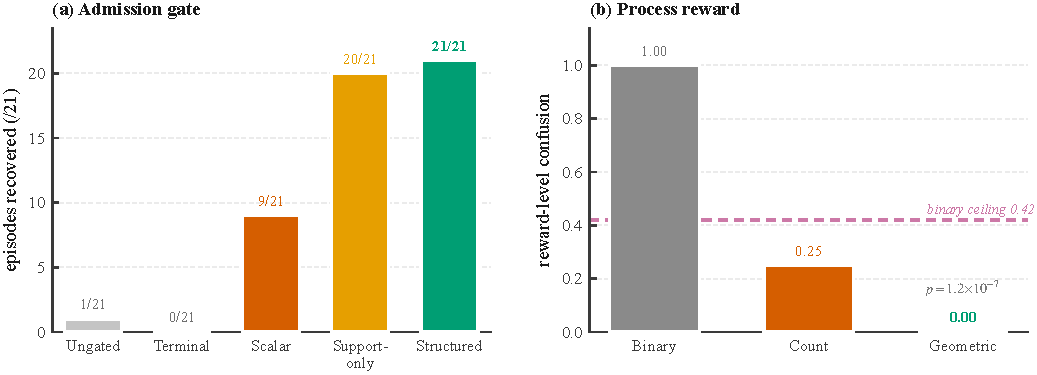
\includegraphics[width=0.84\textwidth]{figures/cand_dual_ladder.pdf}
\caption{One product order, two design points. (a)~As a runtime admission gate at matched $N{=}7$, the product order recovers $\mathbf{21/21}$ multi-action episodes, where support-only (Grid-Agent) reaches $20/21$, the best scalar slack $9/21$, ungated $1/21$, and terminal $0/21$. (b)~As a GRPO process reward, the same geometry has zero reward-level confusion against $0.25$ for its count projection and $1.0$ for a binary signal (oracle-optimal binarization ceiling $0.42$); the dominance holds in all $24$ mined scenarios (sign test $p{=}1.2{\times}10^{-7}$). Scalar projection loses the geometry at both design points.}
\label{fig:dualladder}
\end{figure*}

\paragraph{RQ1: binary terminal admission deadlocks recovery.}
Figure~\ref{fig:dualladder}(a) reports the headline recovery ladder at matched $N{=}7$ ($21$ episodes/policy). Terminal recovers $0/21$ (rejection rate $1.000$): it rejects every intermediate proposal because $S(\hat{s}_{t+1})\ne\emptyset$ at every proposed step, regardless of search depth. Structured admission recovers $\mathbf{21/21}$ (residual $0.000$) against the scalar sweep peak's $9/21$; the gap is structural rather than sampling noise, significant at the scenario level on the full band (RQ2). The lift is structural: support geometry closes the recovery gap, while the per-branch predicate $\psithree$ adds the severity containment RQ4 requires.

\paragraph{RQ2: scalar admission is insufficient.}
If the terminal gate fails only because it is too strict, the natural fix is to admit any proposal whose aggregate penalty $P$ is within a small slack. Relaxing the threshold neither closes the gap nor improves monotonically: across $\eta\in\{0,0.05,0.10,0.20\}$ recovery is $5/21,9/21,7/21,7/21$ (each far below structured admission's $21/21$). The non-monotonicity is itself a trap signature: the $\eta{=}0.05\!\to\!0.10$ drop comes entirely from Scenario~A and Scenario~C, where wider slack admits an early $P$-improving proposal and commits to a residual plateau---wider slack recovers \emph{less} because admission is a commitment operator: on Scenario~A/Scenario~C a wider slack admits the first $P$-improving proposal and commits to a plateau rather than rejecting it to keep the per-step search alive. Were recovery monotone in slack the trap would be falsified; the observed reversal is its signature. The lift comes from support geometry, not magnitude: $\psione\wedge\psitwo$ recovers $20/21$ and the full gate $21/21$. The scalar gap is consistent with Prop.~\ref{prop:gap}: it localizes to the $\preceq$-incomparable geometry of Scenario~A/Scenario~C that no scalar surrogate can order. The full $24$-scenario band confirms this (Table~\ref{tab:band24}): structured admission recovers $\mathbf{120/120}$ against the best scalar gate's $96/120$ (terminal deadlocks); treating each of the $24$ scenarios as an independent cluster, the structured-vs-scalar advantage is significant (scenario-clustered Wilcoxon $p{=}0.004$, bootstrap 95\% CI on the gap excluding zero).

\begin{table}[t]
\centering
\caption{RQ2: full $24$-scenario band ($24$ mined multi-action scenarios), $N{=}5$, recovery [Wilson 95\% CI]. Structured admission recovers the band; the scalar gap localizes to geometry-poor points; terminal deadlocks (Support-only is the Grid-Agent rollback baseline).}
\label{tab:band24}
\footnotesize
\begin{tabular*}{\columnwidth}{@{\extracolsep{\fill}}lcc@{}}
\toprule
Policy & Recovery & 95\% CI \\
\midrule
Terminal                            & $0/120$  & $[0.00,0.03]$ \\
Scalar$_{\eta=0.05}$      & $96/120$ & $[0.72,0.86]$ \\
Support-only                            & $113/120$ & $[0.88,0.97]$ \\
Structured                       & $\mathbf{120/120}$ & $\mathbf{[0.97,1.00]}$ \\
\bottomrule
\end{tabular*}
\end{table}

\paragraph{RQ3: the projection-trap plateau is gate-induced.}
The trap predicts a per-trace signature: the scalar gate accepts one early locally-improving proposal and plateaus while structured admission clears the scenario. It appears across the ordered triple (scalar at its per-scenario best $\eta$): Scenario~B is smooth (scalar $7/7$, residual $0.00$); Scenario~C plateaus at $\le2/7$ (residual $5.94$ vs.\ default $17.59$) against structured $7/7$; Scenario~A is harder still ($\le1/7$) against structured $7/7$ (Fig.~\ref{fig:trap}). Providing the scalar-admitted Scenario~C plateau to an MPC feasibility oracle (constant-setpoint baseline) recovers it to zero penalty in one rollout, confirming the plateau is gate-induced rather than an unrecoverable state: the structured gate avoids it by declining the geometry-poor first step.

\begin{figure}[t]
\centering
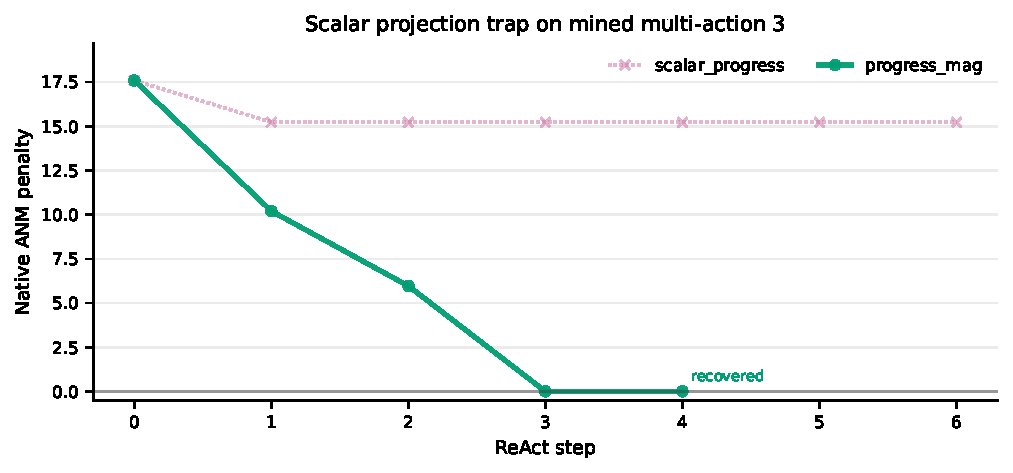
\includegraphics[width=\columnwidth]{figures/fig_trap_multi3.pdf}
\caption{Scalar projection trap on Scenario~C. Structured admission descends to recovery $\Phi(s){=}(\emptyset,\mathbf{0})$ via accepted \texttt{SAFE\_PROGRESS} steps, whereas the scalar gate admits one early locally-improving proposal and plateaus at nonzero residual across all four slack settings (best $2/7$ at $\eta{=}0.05$).}
\label{fig:trap}
\end{figure}

\paragraph{RQ4: trust-boundary containment under LLM-side compromise.}
A mini-suite covers three attack families in four configurations (prompt injection, observation poisoning, and stall in plain and RAG forms) across the three mined scenarios, plus a matched benign control ($60$ attack $+\,15$ benign $=75$ episodes). It records zero safety failures: $0/60$ attack success, false recovery, and material worsening on attacked episodes, and $0/15$ on benign controls. Containment is \emph{architectural}, since the verifier never accesses the LLM's prompt or observation channels (Prop.~\ref{prop:inv}).

\paragraph{The per-branch predicate $\psithree$ is necessary.}
The mini-suite establishes containment against channel compromise; whether the per-branch predicate is \emph{necessary} is a separate question, isolated by a dedicated $120$-case suite. \emph{Magnitude redistribution} (C1/C2) drives one retained branch toward failure while holding the overloaded-branch set and the aggregate penalty within nominal bounds, evading aggregate- and support-level monitoring. Across this suite a scalar gate is breached $43/120$ and the support-only Grid-Agent rollback baseline ($\psione\wedge\psitwo$) $11/120$, whereas the full gate ($\psione\wedge\psitwo\wedge\psithree$) is breached $0/120$ (Fig.~\ref{fig:breach}): only the per-branch test $\psithree$ rejects the concentrating step.

\begin{figure}[t]
\centering
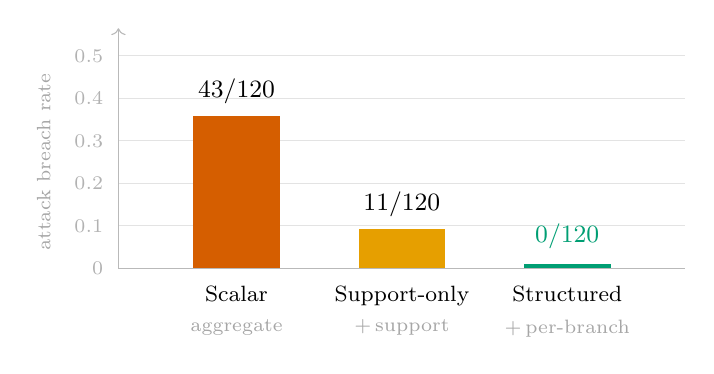
\begin{tikzpicture}[font=\sffamily]
  \def\axw{7.2}
  \def\axh{2.7}
  \def\ymax{0.5}
  \pgfmathsetmacro{\sy}{\axh/\ymax}
  \def\bw{1.1}
  \foreach \r in {0,0.1,0.2,0.3,0.4,0.5}{
    \pgfmathsetmacro{\yy}{\r*\sy}
    \draw[gray!22] (0,\yy) -- (\axw,\yy);
    \node[gray!60,font=\scriptsize,left=2pt] at (0,\yy) {\pgfmathprintnumber[fixed,precision=1]{\r}};
  }
  \draw[->,gray!55] (0,0) -- (0,\axh+0.35);
  \draw[gray!55] (0,0) -- (\axw,0);
  \node[gray!70,font=\scriptsize,rotate=90] at (-0.95,\axh/2) {attack breach rate};
  \pgfmathsetmacro{\ha}{0.358*\sy}
  \fill[oiVermillion] (1.5-\bw/2,0) rectangle (1.5+\bw/2,\ha);
  \node[font=\small\bfseries,above=1pt] at (1.5,\ha) {$43/120$};
  \node[font=\footnotesize,below=3pt] at (1.5,0) {Scalar};
  \node[gray!70,font=\scriptsize,below=15pt] at (1.5,0) {aggregate};
  \pgfmathsetmacro{\hb}{0.092*\sy}
  \fill[oiOrange] (3.6-\bw/2,0) rectangle (3.6+\bw/2,\hb);
  \node[font=\small\bfseries,above=1pt] at (3.6,\hb) {$11/120$};
  \node[font=\footnotesize,below=3pt] at (3.6,0) {Support-only};
  \node[gray!70,font=\scriptsize,below=15pt] at (3.6,0) {$+$\,support};
  \fill[oiGreen] (5.7-\bw/2,0) rectangle (5.7+\bw/2,0.055);
  \node[font=\small\bfseries,above=2pt,text=oiGreen] at (5.7,0.055) {$0/120$};
  \node[font=\footnotesize,below=3pt] at (5.7,0) {Structured};
  \node[gray!70,font=\scriptsize,below=15pt] at (5.7,0) {$+$\,per-branch};
\end{tikzpicture}
\caption{RQ4: magnitude-redistribution breach rate by admission tier---each added predicate closes more attack surface: Scalar $43/120$, Support-only (Grid-Agent, $\psi_1\wedge\psi_2$) $11/120$, Structured ($\psi_1\wedge\psi_2\wedge\psi_3$) $0/120$.}
\label{fig:breach}
\end{figure}

\paragraph{Strong scalar baselines on the full witness pool.}
Beyond the support-preserving redistribution of Fig.~\ref{fig:breach}, full-pool enumeration surfaces the complementary Prop.~\ref{prop:gap} antichain---support expansion---and confirms the gap is representational. Over all $558$ physically-unsafe one-step actions in ANM, the sup-norm $\|\sigma\|_\infty$ admits $46$ and a lexicographic order on $(|S|,\sum_i\sigma_i)$ admits $88$ (instances of the antichain: a new branch overloads while $\max_i\sigma_i$ falls), while the full product order admits $0/558$. The same class recurs in CityLearn over $11{,}311$ physically-unsafe actions under an independent state-of-charge/feeder oracle (verifier-level enumeration, no LLM, so the gate is independent of model choice): the sup-norm admits $6761$, the full gate $0/11{,}311$ (RQ5 gives the full ReAct-loop replication). Counts differ across pools because the witness categories differ; the invariant comparison is zero-versus-nonzero---only the full product order admits none in both domains (supplement).

\paragraph{RQ5: generalization across families and a second domain.}
At the ReAct level, the terminal-versus-structured dichotomy is family-independent and transfers across domains (Table~\ref{tab:gen}): across Qwen3 (two sizes), Gemma-3~\citep{gemma3}, and Llama-3.1~\citep{llama3} on ANM, terminal deadlocks every model ($0/15$) while structured admission recovers completely ($15/15$). The same admission-semantics pattern recurs in CityLearn building-energy dispatch~\citep{citylearn}: the terminal predicate clears only the single-step scenario and deadlocks the multi-step ones, while structured admission recovers broadly. Admission semantics port intact---the verifier-level predicate grades and contains independently of model choice---while recovery completion tracks model capability (Table~\ref{tab:gen}): \emph{structural portability} of the gate semantics in a distinct physical model.

\begin{table}[t]
\centering
\caption{RQ5: generalization across model families (ANM) and to a second domain (CityLearn), $N{=}5$ (recovery). Terminal deadlocks multi-step recovery in both domains (clearing only the single-step CityLearn scenario, $5/15$); Structured admission recovers ANM fully and the CityLearn multi-step scenarios, completion model-dependent. CityLearn at $C_{\text{step}}{=}8$; $^\ast$Qwen3-8B reaches $15/15$ at $C_{\text{step}}{=}16$. ANM Structured per-model ($3$ scenarios pooled) Wilson 95\% CI $[0.80,1.00]$.}
\label{tab:gen}
\footnotesize
\setlength{\tabcolsep}{5pt}
\begin{tabular*}{\columnwidth}{@{\extracolsep{\fill}}lcccc@{}}
\toprule
 & \multicolumn{2}{c}{ANM} & \multicolumn{2}{c}{CityLearn} \\
\cmidrule(lr){2-3}\cmidrule(lr){4-5}
Model & Term. & Structured & Term. & Structured \\
\midrule
Qwen3-8B     & $0/15$ & $\mathbf{15/15}$ & $5/15$ & $14/15^\ast$ \\
Qwen3-14B    & $0/15$ & $\mathbf{15/15}$ & $5/15$ & $\mathbf{15/15}$ \\
Gemma-3-12B  & $0/15$ & $\mathbf{15/15}$ & $5/15$ & $10/15$ \\
Llama-3.1-8B & $0/15$ & $\mathbf{15/15}$ & $5/15$ & $\mathbf{15/15}$ \\
\bottomrule
\end{tabular*}
\end{table}

\section{From Admission Gate to Process Reward}
\label{sec:reward}

\begin{figure*}[t]
\centering

\includegraphics[width=0.92\textwidth]{figures/train_enhancement.pdf}
\caption{Training dynamics in the multi-family stress regimes. (a)~Coupling regime: the geometric reward converges to full recovery within five GRPO iterations, while the count reward---blind to the cross-family drift its own actions cause---is driven below its random initialization: maximizing cleared count actively teaches the policy to sacrifice the fragile family. (b)~Trained recovery versus $\sigma$-heterogeneity: the severity scalar's failure emerges at $\sigma_L/\sigma_S\!\approx\!4$ and saturates from $8$ onward, with CityLearn's measured ratio ($286$, dashed) deep inside the collapsed regime; the homogeneous limit (all arms tie) shows the failure is caused by heterogeneity, not the construction.}
\label{fig:trainenh}
\end{figure*}

The product order is the right structure at a \emph{second design point}: not only the criterion a runtime gate admits on, but the unit a policy should \emph{internalize}. We reuse the identical verifier---its graded verdict and the persisted branch state $\Phi$ of Eq.~\ref{eq:phi}---as a process reward for GRPO~\citep{deepseekmath2024grpo,lightman2024prm}, without changing the verifier or adding task-specific outcome labels, fine-tuning Qwen3-8B with LoRA on the $9$ hardest multi-action ANM scenarios (those the ungated base does not fully recover). Our primary outcome is \emph{ungated} recovery: the gate is removed at evaluation, so recovery measures what the policy internalized rather than what the gate enforces.

\paragraph{The geometry is a higher-fidelity process reward.}
We measure reward-layer fidelity directly, scoring every legal single-setpoint action at each trap state against the true one-step recovery value. The geometric reward never mis-orders a genuinely-different action pair (reward-level confusion $0.000$), strictly dominating its count projection's $0.25$ in all $24$ mined scenarios (sign test $p{=}1.2{\times}10^{-7}$), while a binary admit/reject signal cannot rank admissible steps at all ($1.0$; Fig.~\ref{fig:dualladder}(b)). The separation is a property of the reward, not the rollout distribution: it persists over the full legal action set ($0.04$ for geometric, $0.19$ for count, $0.63$ for the binary signal) and holds even against an oracle-optimal binarization of the true value---the limit of a process reward trained on binary outcome labels~\citep{lightman2024prm}, which still confuses $0.42$. The geometric ranking matches the oracle at Spearman $\rho{=}0.986$. Its robustness to on-policy, complexity-scaling, and reward-noise controls is reported in the supplementary material; we next evaluate policy optimization under these reward signals.

\paragraph{Geometry is the active ingredient.}
Three reward arms share the same rollout gate and differ only in the signal. The full geometric reward---descent in the product order over $\Phi$---is the only one under which the trained policy stays above the untrained base once the gate is removed ($\mathbf{0.844}$ vs.\ $0.778$); stripping the geometry to a verdict ladder ($0.733$) or a violation count ($0.667$) leaves the policy \emph{worse} than untrained, indicating gate-dependent behavior rather than internalized recovery (gated recovery and step counts in the supplementary material). On $15$ held-out scenarios disjoint from training the geometric policy recovers $14/15$ ungated against the base's $9/15$ (one-sided Fisher exact $p{=}0.04$), carrying the geometry to unseen instances.

\paragraph{The same scalarization gap, on the training side.}
This is the training-side counterpart of the admission-side impossibility: the scalarization that is unsound as an admission rule (Prop.~\ref{prop:gap}) collapses the GRPO advantage signal as a reward.
\begin{proposition}[Advantage collapse]
\label{prop:collapse}
With $B$ concurrent violation branches, a count-based reward takes at most $B{+}1$ distinct values, so action pairs within a count-equivalence class receive identical immediate reward---no step-level advantage separation; and along a continuous partial reduction of any single branch the count reward is piecewise constant (zero gradient except at elimination points), whereas the graded geometric reward is strictly monotone in that reduction.
\end{proposition}

\noindent Empirically the flat fraction of the count reward is $98\%$ of the continuous action range (proof in the supplementary material), inducing a \emph{failure class}: with several physically incomparable violation families active, every tested scalar projection of the reward fails to train recovery in at least one regime. We isolate the mechanism in a controlled tabular GRPO setting (Table~\ref{tab:failureclass}; $16$ training seeds each, the same analytic reward forms used above, policy class and regime design in the supplementary material). In a $\sigma$-heterogeneity regime the severity scalar is dominated by raw magnitude and recovers $0\%$; in a coupling regime the count reward is blind to the cross-family drift its own actions cause and trains to $12\%$ (Fig.~\ref{fig:trainenh}(a)). Each scalar augmentation closes only one regime---a drift term rescues count under coupling ($1.00$) but not cross-family priority ($0.80$)---while the full geometry is robust in both.

\paragraph{The collapse is a threshold effect that reproduces at scale.}
The severity-scalar failure emerges at $\sigma_L/\sigma_S\!\approx\!4$ and CityLearn's measured ratio ($286$) lies deep in the collapsed regime (Fig.~\ref{fig:trainenh}(b)); further coupling--floor grids and an MLP policy reproduce the ordering. In a four-building multi-family CityLearn stress suite (Qwen3-8B, GRPO; supplementary material), the geometric reward's advantage tracks the measured one-step action value at Spearman $\rho{=}0.96$ versus $0.79$ for count, and the count arm leaves the battery family with $14\%$ higher residual severity at matched violation count---the signature of a severity-blind signal.

\begin{table}[t]
\centering
\caption{The scalarization failure class: trained recovery in the two multi-family stress regimes ($16$ seeds each). Every scalar projection fails in at least one regime; the full product-order geometry is robust in both.}
\label{tab:failureclass}
\footnotesize
\begin{tabular*}{\columnwidth}{@{\extracolsep{\fill}}lcc@{}}
\toprule
 & \multicolumn{2}{c}{trained recovery} \\
\cmidrule(lr){2-3}
Training reward & $\sigma$-het & coupling \\
\midrule
\textbf{geometric (full $\Phi$)} & $\mathbf{1.00}$ & $\mathbf{1.00}$ \\
severity-scalar ($\Sigma\sigma$ descent) & $0.00$ & $0.04$ \\
count ($|S|$ descent) & $0.80$ & $0.12$ \\
count with drift penalty & $0.80$ & $1.00$ \\
\bottomrule
\end{tabular*}
\end{table}

\section{Conclusion}
\label{sec:conclusion}

We studied runtime governance for LLM tool-calling agents under \emph{post-violation recovery admission} and identified the \emph{scalar projection trap}: a scalar gate, as a search operator over the ReAct stream, commits the trajectory to a residual plateau. We support this with a representational impossibility (Prop.~\ref{prop:gap}), an LLM-independent admission invariant (Prop.~\ref{prop:inv}), and an empirical falsifier---structured admission recovers $21/21$ where the best scalar slack reaches $9/21$ and terminal stalls at $0/21$---holding across three model families and a second domain. Under the C1--C3 compromised-LLM adversary, only the full per-branch predicate contains a magnitude-redistribution attack that defeats both scalar and Grid-Agent baselines. Reused as a GRPO process reward, the same product-order geometry is the only signal that keeps the policy above the untrained baseline once the gate is removed. Scalarization loses the geometry at both design points; only the full product order is structurally sufficient.

\bibliography{refs}

\appendix
\section{Reproducibility Checklist}

\noindent\textbf{This paper:}
\begin{itemize}\setlength{\itemsep}{0pt}
\item Includes a conceptual outline and/or pseudocode description of AI methods introduced --- \textbf{yes}.
\item Clearly delineates statements that are opinions, hypothesis, and speculation from objective facts and results --- \textbf{yes}.
\item Provides well-marked pedagogical references for less-familiar readers --- \textbf{yes}.
\end{itemize}

\noindent\textbf{Does this paper make theoretical contributions? yes.}
\begin{itemize}\setlength{\itemsep}{0pt}
\item All assumptions and restrictions are stated clearly and formally --- \textbf{yes}.
\item All novel claims are stated formally --- \textbf{yes} (Props.~1--3).
\item Proofs of all novel claims are included --- \textbf{yes} (Prop.~1 in the main text; Props.~2--3 in the supplementary material).
\item Proof sketches or intuitions are given for complex/novel results --- \textbf{yes}.
\item Appropriate citations to theoretical tools used are given --- \textbf{yes}.
\item All theoretical claims are demonstrated empirically to hold --- \textbf{yes}.
\item All experimental code used to eliminate or disprove claims is included --- \textbf{partial} (released upon publication).
\end{itemize}

\noindent\textbf{Does this paper rely on one or more datasets? yes.}
\begin{itemize}\setlength{\itemsep}{0pt}
\item A motivation is given for why the experiments are conducted on the selected datasets --- \textbf{yes}.
\item All novel datasets introduced are included in a data appendix --- \textbf{partial} (the scenario pool is generated by the described mining procedure over public benchmarks).
\item All novel datasets will be made publicly available upon publication --- \textbf{yes}.
\item All datasets drawn from existing literature are accompanied by appropriate citations --- \textbf{yes}.
\item All datasets drawn from existing literature are publicly available --- \textbf{yes} (Gym-ANM, CityLearn).
\item All datasets that are not publicly available are described in detail --- \textbf{NA}.
\end{itemize}

\noindent\textbf{Does this paper include computational experiments? yes.}
\begin{itemize}\setlength{\itemsep}{0pt}
\item States the number and range of values tried per (hyper-)parameter and the selection criterion --- \textbf{partial} (admission $\alpha,\varepsilon$ and scalar slack $\eta$ swept; GRPO settings in the supplementary material).
\item Code required for pre-processing data is included --- \textbf{partial} (upon publication).
\item All source code for conducting and analyzing experiments is included --- \textbf{partial} (upon publication).
\item All source code will be made publicly available upon publication --- \textbf{yes}.
\item Source code implementing new methods has comments detailing the implementation --- \textbf{yes}.
\item If an algorithm depends on randomness, the method for setting seeds is described --- \textbf{partial} (results pooled over the stated number of training seeds; seed values released with the code).
\item Specifies the computing infrastructure (hardware and software) --- \textbf{partial} (vLLM-served open-weight LLMs; single-CPU-core verifier timing reported; further hardware/software details released with the code).
\item Formally describes evaluation metrics and the motivation for choosing them --- \textbf{yes} (recovery, attack-breach, with Wilson intervals).
\item States the number of algorithm runs used to compute each reported result --- \textbf{yes}.
\item Analysis goes beyond single-dimensional summaries to include variation/confidence --- \textbf{yes} (Wilson 95\% CIs throughout).
\item The significance of any improvement is judged using appropriate statistical tests --- \textbf{yes} (scenario-clustered bootstrap and Wilcoxon; one-sided Fisher exact).
\item Lists all final (hyper-)parameters used --- \textbf{partial} (main text and supplementary material).
\end{itemize}

\end{document}
